\title{
\centering

\includegraphics[width=4cm,height=4cm,keepaspectratio]{du.jpg} \\ \ CSE - 4255 Data Mining and Warehousing Lab\\  \Large \textit{Comparison Between the Performance of K - Means and K - Medoids Algorithm in Clustering}\\}


\author{
        Saif Mahmud \\
        Roll: SH - 54\\
            \and
        M. Tanjid Hasan Tonmoy\\
        Roll: SH - 09\\
            \and
        \\\textbf{Submitted To:}\\ Dr. Chowdhury Farhan Ahmed \\
        Professor\\
        \\ \& \\ 
        Abu Ahmed Ferdaus\\
        Associate Professor\\ \\
        Department of Computer Science and Engineering\\
        University of Dhaka        
}
\date{\today}

\documentclass[12pt]{article}
\usepackage{graphicx}
\usepackage{cite}
\usepackage{url}
\usepackage{multirow}
\usepackage{longtable}
\usepackage{multirow}
%\usepackage[a4paper]{geometry}
\newcommand{\s}{\vspace{0.2cm}}
\usepackage{float}

\begin{document}


\maketitle
\thispagestyle{empty}
\clearpage
\newpage

\section{Problem Definition}

\section{Dataset Description}

\section{Theory and Implementation}
\subsection{K - Means}
\subsection{K - Medoids}

\section{Evaluation of Clustering}

\subsection{Elbow Method}

\begin{figure}[H]
	\centering
	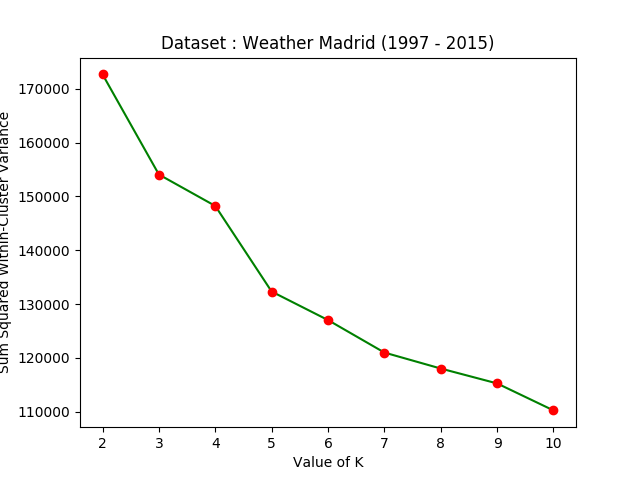
\includegraphics[width = \linewidth, height = 10.5cm]{Elbow_Weather.png}
	\caption{Determining Value of K through Elbow Method (K - Means)}
	\label{fig:elbow_weather}
\end{figure}

\begin{figure}[H]
	\centering
	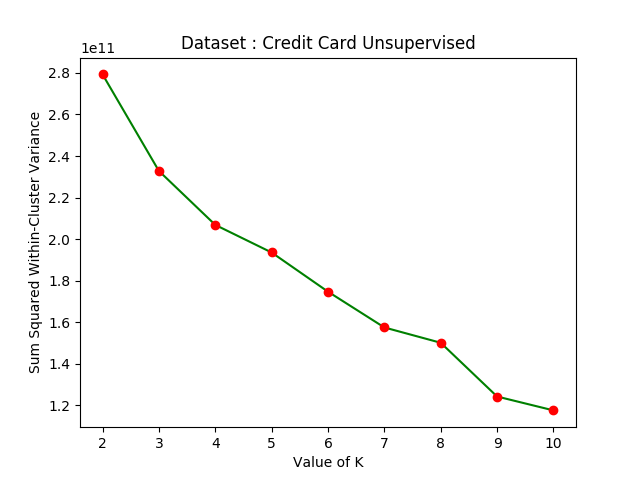
\includegraphics[width = \linewidth, height = 10.5cm]{Elbow_CreditCard.png}
	\caption{Determining Value of K through Elbow Method (K - Means)}
	\label{fig:elbow_credit}
\end{figure}

\subsection{Time Complexity Comparison}

\begin{figure}[H]
	\centering
	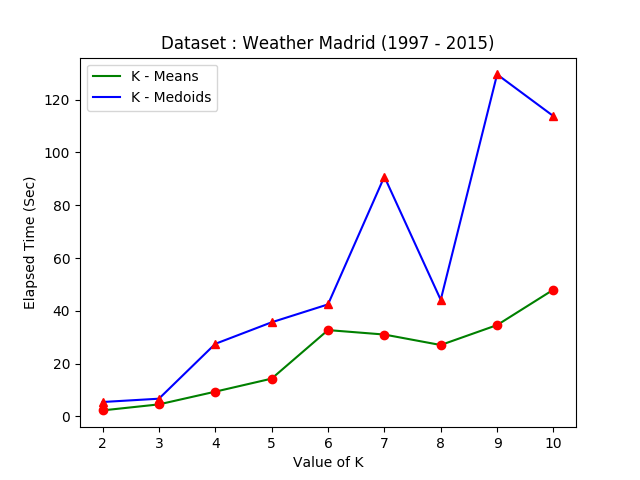
\includegraphics[width = \linewidth, height = 10.5cm]{Weather.png}
	\caption{Comparison of Elapsed Time between K - Means and K - Medoids Algorithm}
	\label{fig:weather}
\end{figure}

\begin{figure}[H]
	\centering
	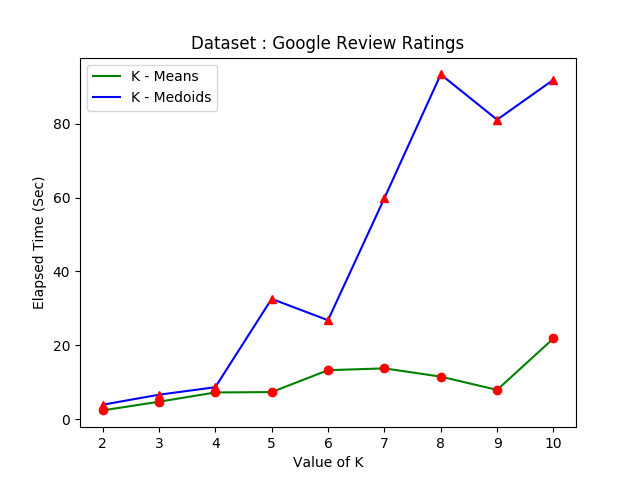
\includegraphics[width = \linewidth, height = 10.5cm]{Google.png}
	\caption{Comparison of Elapsed Time between K - Means and K - Medoids Algorithm}
	\label{fig:google}
\end{figure}

\begin{figure}[H]
	\centering
	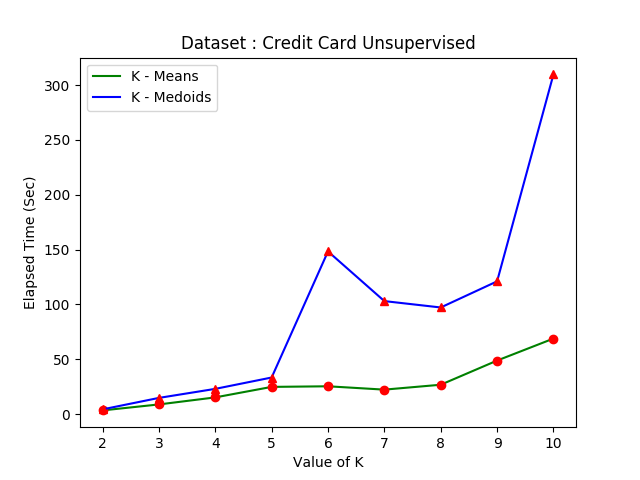
\includegraphics[width = \linewidth, height = 10.5cm]{CreditCard.png}
	\caption{Comparison of Elapsed Time between K - Means and K - Medoids Algorithm}
	\label{fig:credit}
\end{figure}



\section{Conclusion}



\end{document}
